\documentclass[letterpaper,10pt,conference]{ieeeconf}
\overrideIEEEmargins

\usepackage[T1]{fontenc}
\usepackage[utf8]{inputenc}
\usepackage{microtype}
\usepackage{amsmath,amssymb,bm}
\usepackage{booktabs,tabularx,array,multirow}
\usepackage{graphicx}
\usepackage{siunitx}
\usepackage{xcolor}
\usepackage{tikz}
\usetikzlibrary{arrows.meta,positioning,fit,calc}
\usepackage{pgfplots}
\pgfplotsset{compat=1.18}
\usepackage{cite}
\usepackage[hidelinks]{hyperref}
\usepackage[nameinlink,capitalize]{cleveref}

\definecolor{rppblue}{HTML}{174A6E}
\definecolor{rppgray}{HTML}{5B6570}

\sisetup{
  detect-all,
  group-separator={,},
  group-minimum-digits=4
}

\newcommand{\RPP}{Robotic Printing Platform}
\newcommand{\se}{\mathrm{SE}(3)}
\newcommand{\RR}{\mathbb{R}}
\newcommand{\software}[1]{\texttt{#1}}

\title{\LARGE\bfseries A Material-Aware Pipeline from Slicer G-code to
Simulation-Ready Robotic Additive-Manufacturing Trajectories}
\author{Author names, affiliations, and contact information to be added}

\hypersetup{
  pdftitle={A Material-Aware Pipeline from Slicer G-code to Simulation-Ready Robotic Additive-Manufacturing Trajectories},
  pdfauthor={Author names and affiliations to be added},
  pdfsubject={Working draft on the Robotic Printing Platform},
  pdfkeywords={robotic additive manufacturing, G-code, inverse kinematics, trajectory retiming, Isaac Sim}
}

\begin{document}
\maketitle
\thispagestyle{empty}
\pagestyle{empty}

% An abstract is intentionally omitted at the authors' request while the
% perception, dynamic-environment, and physical-validation studies are added.
\noindent\textit{\textbf{Draft status---}
This manuscript documents the planning, validation, export, and deposition
functionality implemented in the repository at the stated date.  Perception,
learned prediction, adaptive control, deformable-surface repair, and physical
printing experiments are planned extensions and are not presented as completed
results.  An abstract will be added after those studies are incorporated.}

\noindent\textbf{Keywords---}robot-assisted additive manufacturing; G-code;
inverse kinematics; trajectory retiming; material-aware deposition; Isaac Sim;
in situ bioprinting.

\section{Introduction}

Material-extrusion slicers normally describe the motion of a Cartesian machine:
the tool position, feed rate, layer, and extrusion state are encoded without a
model of a serial manipulator.  A robot arm adds joint limits, kinematic
redundancy, singular configurations, self- and workcell-collision risks, a
calibrated tool-center point (TCP), and a trajectory controller whose realized
motion can differ from its command.  Consequently, forwarding conventional
G-code directly to a robot does not establish that the path is reachable,
dynamically admissible, or suitable for simulation.

Robot-assisted additive manufacturing (AM) is attractive because additional
degrees of freedom can enlarge the work envelope and enable multidirectional or
conformal deposition, but the same flexibility increases process-planning and
integration complexity~\cite{urhal2019robot,bhatt2020expanding}.  In situ
bioprinting makes this gap especially visible: prior systems have projected
paths onto irregular anatomy, compensated periodic patient motion, and combined
multiple tools and materials~\cite{fortunato2021platform,fortunato2022motion,
guerra2025multimaterial}.  These studies motivate a modular software substrate
on which sensing and closed-loop repair can later be evaluated without
conflating unimplemented intelligence with the lower-level planning and
deposition stack.

This paper presents the current \RPP{}, an offline Python toolchain that converts
modal Cura/Marlin-style G-code into material-aware Cartesian waypoints, solves a
URDF-defined serial manipulator, retimes and validates the joint trajectory, and
exports a portable NVIDIA Isaac Sim replay.  The contribution is an integrated,
inspectable platform rather than a claim of a new inverse-kinematics algorithm,
a calibrated constitutive material law, or a physical printing result.  The
implemented contributions are:

\begin{enumerate}
  \item an explicit sequence of parser, path, robot, retiming, validation, and
  exporter contracts that supports Franka Panda, UR5, and UR5e packages;
  \item preservation of layer, feed, print/travel, run, and extrusion metadata
  through collinearity simplification and path densification, with fail-fast
  extrusion conservation and three configurable interpretations of G-code
  \(E\);
  \item weighted damped-least-squares IK with free nozzle-yaw sampling, greedy
  or second-order dynamic-programming selection, constraint-aware retiming, and
  machine-readable trajectory diagnostics; and
  \item simulator-independent deposition driven by measured TCP samples and an
  exact piecewise volumetric-flow schedule, with geometric and PhysX
  position-based-dynamics (PBD) replay backends.
\end{enumerate}

We evaluate the present working tree in two ways.  First, a common
\SI{25}{\milli\meter} by \SI{15}{\milli\meter} volumetric patch is planned for
all three robot packages with the same 446 Cartesian waypoints.  Second, we
audit an archived full-resolution UR5e first-layer planning snapshot containing
13,099 waypoints.  We also report a fresh pass of all 55 automated tests and
state the boundary between source-level verification, qualitative Isaac replay,
and evidence that does not yet exist.

\section{Related Work}

\subsection{Robotic additive manufacturing}

Reviews of robotic AM identify multidirectional fabrication, conformal
deposition, support reduction, assembly, and large-scale production as central
capabilities enabled by articulated systems~\cite{urhal2019robot,
bhatt2020expanding}.  Their recurring challenges---path representation,
kinematic feasibility, process coordination, collision checking, and
robot-specific integration---suggest that a useful research platform should
separate manufacturing intent from a particular manipulator or simulator.
The present work follows that separation: G-code and process metadata are
represented independently of the serial-chain solver, while robot geometry and
limits live in replaceable packages.

\subsection{In situ and adaptive bioprinting}

Fortunato et al. developed a five-degree-of-freedom platform and path-planning
workflow for deposition on irregular surfaces~\cite{fortunato2021platform}.
Their later system used vision to compensate physiological motion and update a
nominal path online~\cite{fortunato2022motion}.  Guerra et al. extended the
same platform toward automated multi-tool, multi-material, and multi-scale
operation~\cite{guerra2025multimaterial}.  These systems demonstrate that
surface geometry, robot motion, and material delivery must ultimately be
coupled.  The \RPP{} currently supplies the offline trajectory and simulation
substrate for such work; it does not yet implement RGB-D reconstruction,
deformable-surface tracking, learned outcome prediction, or model-predictive
control.

\subsection{Kinematic and particle-simulation foundations}

The robot solver uses a damped Jacobian inverse, a classical approach for
reducing numerical sensitivity near singular configurations~\cite{
nakamura1986singularity}.  It reports the product of Jacobian singular values as
Yoshikawa manipulability and also retains the smallest singular value as a more
direct local conditioning indicator~\cite{yoshikawa1985manipulability}.  URDF
provides the serial-chain description used by the dependency-light kinematics
layer; its role within ROS is documented by Quigley et al.~\cite{quigley2009ros}.

For replay, the project uses either explicit geometric beads or PhysX PBD
particles.  PBD updates positions through constraints rather than integrating a
complete force-based constitutive law~\cite{muller2007pbd}; unified particle
formulations extend that principle to fluids, deformables, and rigid bodies in
real-time graphics~\cite{macklin2014unified}.  Accordingly, the platform's PBD
coefficients are treated as simulator controls, not laboratory viscosity or
surface-tension measurements~\cite{nvidia2025particles}.

\section{System Architecture and Scope}

\Cref{fig:architecture} shows the implemented data flow.  Three primary inputs
are resolved at the start of a run: a modal G-code program, a material profile,
and a robot/workcell configuration.  Each stage consumes and enriches explicit
records instead of relying on shared simulator state.  Isaac Sim is therefore
optional for parsing, planning, IK, retiming, validation, and bundle generation.

\begin{figure*}[!t]
\centering
\resizebox{0.98\textwidth}{!}{%
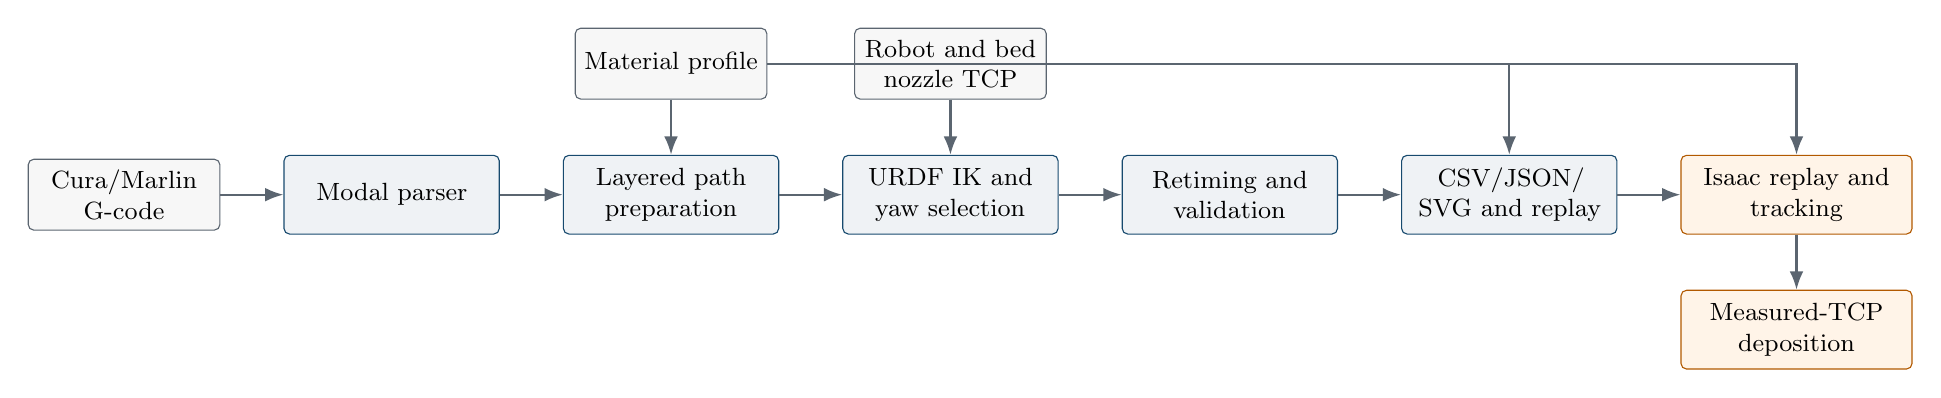
\begin{tikzpicture}[
  node distance=7mm and 8mm,
  >=Latex,
  stage/.style={draw=rppblue,rounded corners=2pt,fill=rppblue!7,
    align=center,minimum height=10mm,text width=25mm,font=\small},
  source/.style={draw=rppgray,rounded corners=2pt,fill=black!3,
    align=center,minimum height=9mm,text width=22mm,font=\small},
  runtime/.style={draw=orange!70!black,rounded corners=2pt,fill=orange!9,
    align=center,minimum height=10mm,text width=27mm,font=\small},
  flow/.style={->,thick,draw=rppgray}
]
  \node[source] (gcode) {Cura/Marlin\\G-code};
  \node[stage,right=of gcode] (parse) {Modal parser};
  \node[stage,right=of parse] (path) {Layered path\\preparation};
  \node[stage,right=of path] (ik) {URDF IK and\\yaw selection};
  \node[stage,right=of ik] (time) {Retiming and\\validation};
  \node[stage,right=of time] (export) {CSV/JSON/\\SVG and replay};
  \node[runtime,right=of export] (isaac) {Isaac replay and\\tracking};
  \node[runtime,below=of isaac] (deposit) {Measured-TCP\\deposition};

  \node[source,above=of path] (material) {Material profile};
  \node[source,above=of ik] (robot) {Robot and bed\\nozzle TCP};

  \draw[flow] (gcode) -- (parse);
  \draw[flow] (parse) -- (path);
  \draw[flow] (path) -- (ik);
  \draw[flow] (ik) -- (time);
  \draw[flow] (time) -- (export);
  \draw[flow] (export) -- (isaac);
  \draw[flow] (isaac) -- (deposit);
  \draw[flow] (material) -- (path);
  \draw[flow] (material.east) -| (export.north);
  \draw[flow] (robot) -- (ik);
  \draw[flow] (robot.east) -| (isaac.north);
\end{tikzpicture}}
\caption{Implemented architecture.  Planning stages operate without Isaac Sim;
the generated replay reads the realized TCP after every physics step and passes
it to a simulator-independent deposition manager.}
\label{fig:architecture}
\end{figure*}

The default operating assumptions are deliberately narrow and inspectable:

\begin{itemize}
  \item linear \software{G0}/\software{G1} Cura/Marlin motion, with modal units,
  positioning, extrusion, and feed state;
  \item selected planar layers recentered on a configured horizontal bed, with
  the nozzle axis globally downward and spin about that axis left free;
  \item one fixed-base serial manipulator described by a URDF chain; and
  \item offline planning and simulator export rather than physical robot
  command or certified real-time control.
\end{itemize}

These assumptions define the evidence in this paper.  Interfaces exist for an
alternative path planner or robot backend, but the presence of an interface is
not evidence that non-planar surface following or hardware execution is already
implemented.

\section{Methods}

\subsection{Modal G-code parsing}

The parser maintains absolute Cartesian position, extrusion state, feed rate,
units, motion mode, extrusion mode, and layer index.  It handles
\software{G20}/\software{G21}, \software{G90}/\software{G91},
\software{M82}/\software{M83}, \software{G92}, \software{G28}, and linear
\software{G0}/\software{G1} moves.  Cura layer comments are preferred; a change
in \(z\) can be used as a fallback layer boundary.  For move \(i\), the parser
retains the absolute extrusion state \(E_i\) and its modal increment
\(\Delta E_i\).  A positive increment marks a printing segment, while travel
and retraction remain represented rather than being discarded.

The sample wall-hook input contains 420,387 parsed moves across 198 commented
layers: 338,468 are classified as printing moves and 81,919 as travel moves.
This parse-scale result should not be confused with the much smaller number of
waypoints used by a capped smoke test.

\subsection{Path preparation and manufacturing metadata}

Moves in the selected layer range are partitioned into contiguous printing and
travel runs.  Near-collinear printing vertices can be removed, but a vertex is
retained when removing it would erase a feed-rate change.  Long segments are
then subdivided to a configured maximum length.  If a segment is divided into
fractions \(\alpha_k\), its extrusion increment is distributed as
\(\Delta E_{i,k}=\alpha_k\Delta E_i\).  The implementation verifies

\begin{equation}
  \sum_{i\in\mathcal{P}} \max(\Delta E_i,0)
  =
  \sum_{k\in\mathcal{W}_{\!P}} \max(\Delta E_k,0)
  \label{eq:extrusion-conservation}
\end{equation}

within a tight floating-point tolerance and aborts if conservation fails.
Here \(\mathcal{P}\) denotes source printing segments and
\(\mathcal{W}_{\!P}\) the prepared printing waypoints.  Every waypoint carries
its base-frame position, nozzle axis, free-yaw flag, layer, run identifier,
feed, raw extrusion increment, material identifier, deposited volume, and
optional mass.

Source \(x\)-\(y\) points are centered, converted from millimetres to metres,
and transformed by a configured bed pose.  The current planner assigns
\(\bm{a}=[0,0,-1]^\mathsf{T}\) as the nozzle axis everywhere.  Non-planar normal
assignment is a future planner, not an active branch of the default algorithm.

\subsection{Material profiles and extrusion conversion}

A strict JSON material profile chooses one of three interpretations of positive
\(E\).  With flow multiplier \(m_f\), filament diameter \(d_f\), and syringe
inner diameter \(d_s\), the deposited volume is

\begin{equation}
  V_i = m_f\max(\Delta E_i,0)
  \begin{cases}
    \pi d_f^2/4, & \text{filament-length mode},\\
    1,            & \text{volumetric mode},\\
    \pi d_s^2/4, & \text{syringe-plunger mode}.
  \end{cases}
  \label{eq:material-volume}
\end{equation}

When density \(\rho\) is present in \si{\gram\per\centi\meter\cubed}, the
estimated mass is \(m_i=\rho V_i/1000\) grams.  The profile is resolved once and
copied into the simulator bundle to prevent an implicit material change between
planning and replay.

The repository contains a conventional PLA profile and a research profile for
an alginate--chitosan polyion-complex formulation.  The formulation and nozzle
context come from Liu et al.~\cite{liu2018alginate}; related alginate extrusion
studies provide rheological and printability context~\cite{gao2024crosslinker,
wang2024handheld,jia2014alginate}.  They do not identify PhysX coefficients.
The current PBD values and visual spreading/shrinkage constants are therefore
transparent starting parameters and heuristics, respectively.

\subsection{URDF kinematics and damped least-squares IK}

The kinematics layer traces fixed, revolute, continuous, and prismatic joints
from the configured base link to the end link.  It evaluates forward kinematics
\(T(\bm q)\in\se\), joint frames, and the geometric Jacobian
\(J(\bm q)\in\RR^{6\times n}\).  The flange-to-nozzle transform is appended to
the URDF chain so the target is the calibrated nozzle TCP rather than the last
robot link.

For desired pose \(T_d\), translational error \(\bm e_p\), rotation-vector
error \(\bm e_R\), orientation weight \(w_R\), and damping \(\lambda\), the
solver forms

\begin{align}
  \bm e &= [\bm e_p^\mathsf{T},\;w_R\bm e_R^\mathsf{T}]^\mathsf{T},\\
  J_w &= \operatorname{diag}(1,1,1,w_R,w_R,w_R)J,\\
  J_\lambda^{\#} &= J_w^\mathsf{T}
  (J_wJ_w^\mathsf{T}+\lambda^2 I)^{-1}.
\end{align}

The bounded update is

\begin{equation}
  \begin{aligned}
  \Delta\bm q ={}& J_\lambda^{\#}\bm e \\
  &+ \eta (I-J_\lambda^{\#}J_w)(\bm q_h-\bm q),
  \end{aligned}
  \label{eq:dls}
\end{equation}

where \(\bm q_h\) is the package home pose and \(\eta\) is a null-space weight.
The second term is projected so that a home-pose preference does not directly
bias the Cartesian objective.  Each iteration limits the infinity norm of
\(\Delta\bm q\) and clamps the result to joint limits.  Success requires both
position and orientation residuals to fall within configured tolerances.

\subsection{Nozzle-yaw selection}

For planar deposition, spin about the nozzle axis is process-redundant but can
change joint motion and conditioning.  The platform uniformly samples candidate
yaws in \([\! -\pi,\pi)\) and solves IK for each sample.  The default greedy mode
selects a candidate using residual and previous-configuration motion.  The
optional global mode operates independently on each deposition run.  Its unary
cost combines weighted residual, a failure penalty, an optional inverse
smallest-singular-value penalty, and an optional collision-warning penalty.

To penalize changes in joint velocity, the dynamic-programming state stores an
ordered pair of adjacent candidate indices.  For a candidate sequence
\(c_1,\ldots,c_N\), retiming estimates \(\Delta t_i\), and joint velocity
\(\bm v_i=(\bm q_{i,c_i}-\bm q_{i-1,c_{i-1}})/\Delta t_i\), the implemented
objective has the form

\begin{equation}
  \begin{aligned}
  C ={}& \sum_{i=1}^{N} U_{i,c_i}
  + w_m\sum_{i=1}^{N}\lVert\bm v_i\rVert_2^2 \\
  &+ w_s\sum_{i=2}^{N}\lVert\bm v_i-\bm v_{i-1}\rVert_2^2.
  \end{aligned}
  \label{eq:dp}
\end{equation}

The repository verifies this recurrence on synthetic candidate sequences.  It
does not yet contain an experimental benchmark showing that global selection
improves a full physical print.

\subsection{Trajectory retiming}

The first segment-duration estimate preserves the G-code feed while respecting
joint velocity limits:

\begin{equation}
  \begin{aligned}
  \Delta t_i^{(0)} = \max\!\Bigg(&
  \frac{\lVert\bm p_i-\bm p_{i-1}\rVert_2}{f_i},\\
  &\max_j\frac{|q_{i,j}-q_{i-1,j}|}{\dot q_j^{\max}},
  10^{-6}\Bigg).
  \end{aligned}
  \label{eq:retime}
\end{equation}

Segment velocities are finite differences.  Internal acceleration is the
centered difference between adjacent segment velocities, while the first and
last accelerations enforce entry from and exit to zero joint velocity.  Forward
and backward passes scale the one or two durations adjacent to a violating
waypoint by the square root of its normalized acceleration excess.  The process
repeats until all configured limits are satisfied or reports failure rather
than silently exporting a violating trajectory.

\subsection{Validation and approximate collision warnings}

The report records IK success, mean/maximum/95th-percentile Cartesian and
rotational residuals, total joint motion, maximum step, velocity and
acceleration violations, joint-limit margin, estimated duration, and material
volume.  It also records Yoshikawa manipulability and the smallest Jacobian
singular value at every waypoint.

Collision diagnostics approximate active robot links by capsules and the bed or
completed material by axis-aligned boxes.  They flag bed clearance,
non-adjacent self-proximity, and tool proximity to completed lower-layer
material.  These sampled, non-blocking warnings are useful for screening but
are neither a continuous collision proof nor a substitute for the collision
models and safety logic of a production controller.

\subsection{Measured-TCP deposition and Isaac replay}

Each trajectory point stores the volume assigned to its incoming segment.  For
\(t_i>t_{i-1}\), the flow schedule uses

\begin{equation}
  Q_i = \frac{V_i}{t_i-t_{i-1}}
  \quad [\si{\milli\meter\cubed\per\second}],
  \label{eq:flow}
\end{equation}

and zero flow for travel.  If a physics step crosses a flow boundary, the
schedule partitions the interval exactly and interpolates intermediate TCP
poses between its two measured endpoints.  This prevents a coarse physics step
from blending printing and travel rates.  Travel samples still refresh the
anchor, so the next printed segment cannot bridge empty space.  A stationary
positive-flow sample produces a droplet; a moving sample emits a segment along
the measured TCP chord.  Position jumps, optional orientation jumps, or time
regressions break continuity and accumulate commanded material as unrepresented
volume rather than drawing across a teleport.

The exporter writes a self-contained replay script, trajectory files, the
resolved material profile, and a copy of the deposition manager.  At runtime,
the replay loads the robot USD, interpolates position targets against the
retimed clock, advances physics, reads the realized TCP from the USD hierarchy,
and then updates deposition.  It also implements desired-versus-actual joint
tracking logs.  No current runtime tracking log is used as evidence in this
paper.

Two deposition sinks share the same schedule and continuity rules.  A visual
sink creates batched USD curves and spherical droplets.  A PhysX sink appends
particles to one shared PBD set and carries fractional particle volume so
discretization does not create systematic loss.  The latter represents gravity,
contact, cohesion, and related solver interactions, but not nozzle heat,
crystallization, curing, acid-induced cross-linking, or a calibrated
thermo-mechanical phase transition.

\subsection{Heuristic bead evolution}

The visual backend can evolve each bead from its immutable birth geometry.  For
age \(t\), asymptotic spreading ratio \(s_\infty\geq1\), spreading time
\(\tau_s\), shrinkage fraction \(\gamma\in[0,1)\), and shrinkage time
\(\tau_v\), it computes

\begin{align}
  s(t) &= 1+(s_\infty-1)(1-e^{-t/\tau_s}),\\
  v(t) &= 1-\gamma(1-e^{-t/\tau_v}),\\
  w(t) &= s(t),\qquad h(t)=\frac{v(t)}{s(t)},\\
  r_{\mathrm{vis}}(t) &= \sqrt{s(t)v(t)}.
  \label{eq:evolution}
\end{align}

Thus \(w(t)h(t)=v(t)\) for an elliptical cross-section with fixed length.
Round curves and spheres use \(r_{\mathrm{vis}}\) as an intentionally coarse
scalar proxy.  \Cref{fig:evolution} plots the current research-profile values
\(s_\infty=1.35\), \(\tau_s=\SI{2}{\second}\), \(\gamma=0.08\), and
\(\tau_v=\SI{30}{\second}\).  The curves visualize configured heuristics, not
measurements of the cited alginate--chitosan formulation.

\begin{figure}[!t]
\centering
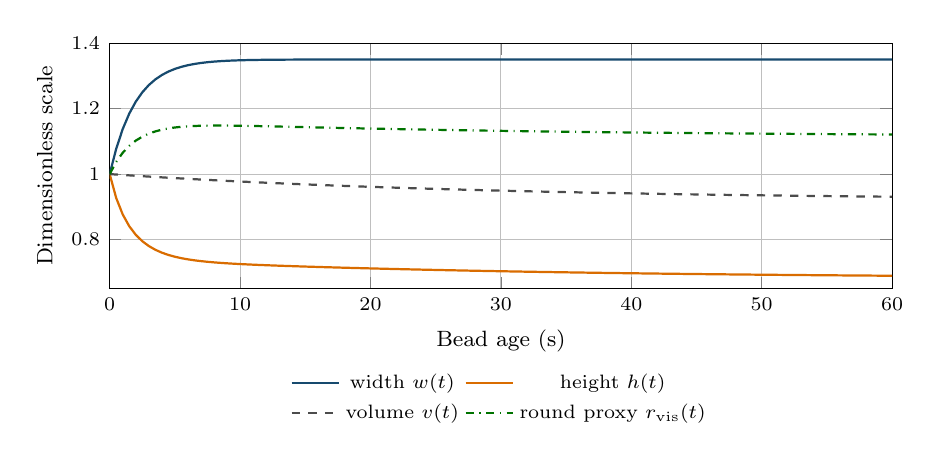
\begin{tikzpicture}
\begin{axis}[
  width=0.95\linewidth,
  height=4.7cm,
  xmin=0,xmax=60,
  ymin=0.65,ymax=1.40,
  xlabel={Bead age (s)},
  ylabel={Dimensionless scale},
  grid=major,
  legend columns=2,
  legend style={at={(0.5,-0.30)},anchor=north,draw=none,font=\scriptsize},
  tick label style={font=\scriptsize},
  label style={font=\footnotesize}
]
  \addplot[rppblue,thick,domain=0:60,samples=121]
    {1+0.35*(1-exp(-x/2))};
  \addlegendentry{width $w(t)$}
  \addplot[orange!85!black,thick,domain=0:60,samples=121]
    {(1-0.08*(1-exp(-x/30)))/(1+0.35*(1-exp(-x/2)))};
  \addlegendentry{height $h(t)$}
  \addplot[black!70,dashed,thick,domain=0:60,samples=121]
    {1-0.08*(1-exp(-x/30))};
  \addlegendentry{volume $v(t)$}
  \addplot[green!45!black,dashdotted,thick,domain=0:60,samples=121]
    {sqrt((1+0.35*(1-exp(-x/2)))*(1-0.08*(1-exp(-x/30))))};
  \addlegendentry{round proxy $r_{\mathrm{vis}}(t)$}
\end{axis}
\end{tikzpicture}
\caption{Configured visual bead-evolution curves.  They expose model behavior
for inspection but are not calibrated rheology or curing data.}
\label{fig:evolution}
\end{figure}

\section{Implementation and Reproducibility}

The offline core targets Python 3.10 or newer and depends only on NumPy.  Isaac
Sim is installed separately and is needed only to execute a generated replay.
The configuration separates robot geometry and limits, bed pose, nozzle TCP,
material, path preparation, and IK parameters.  \Cref{tab:robots} summarizes
the included packages.  All three use the same generic URDF planner API.

\begin{table*}[!t]
\centering
\caption{Bundled robot packages.  Reach is a configured screening value, not a
complete reachable-workspace characterization.}
\label{tab:robots}
\footnotesize
\begin{tabularx}{\textwidth}{@{}lrrX@{}}
\toprule
Package & DoF & Nominal reach & Package-specific role \\
\midrule
Franka Panda & 7 & \SI{0.855}{\meter} & Redundant serial arm and default configuration. \\
UR5 & 6 & \SI{0.85}{\meter} & UR-style chain and simulator asset reference. \\
UR5e & 6 & \SI{0.85}{\meter} & Custom mounted-extruder USD, CAD-derived TCP, and \SI{2}{\milli\meter} position tolerance. \\
\bottomrule
\end{tabularx}
\end{table*}

Each successful run creates a robot-specific bundle containing flat and
structured trajectories, the resolved material profile, a validation report,
top/side path plots, a joint plot, the deposition manager, and the Isaac replay.
The CSV includes pose, layer/run metadata, extrusion, residual, iteration,
Jacobian, time, joint position, velocity, and acceleration fields.  A new robot
normally requires a URDF and JSON package rather than a new solver class; a new
material normally requires one validated JSON profile.

The paper's common-input metrics are archived in
\software{paper/data/compact\_patch\_metrics.csv}.  They were reproduced on
Windows with Python 3.12.13 and NumPy 2.3.5 using the following settings:
volumetric research profile, layer 0, \SI{1}{\milli\meter} maximum segment
length, no angular simplification, and greedy yaw selection.  The input file
explicitly declares that \(E\) is in cubic millimetres.  Panda and UR5 were run
together; UR5e was run separately with the mounted-extruder USD.  Exact commands
are given in the paper-folder README.

\section{Evaluation}

\subsection{Common volumetric patch across three robots}

The compact input contains 16 parallel printed lines over a
\SI{25}{\milli\meter} by \SI{15}{\milli\meter} footprint.  Path preparation
produced 446 waypoints: 416 printing and 30 travel, grouped into 16 deposition
runs.  All robots received the same base-frame Cartesian path and
\SI{64}{\milli\meter\cubed} volume command.  \Cref{tab:compact-results}
reports current-code results.

\begin{table*}[!t]
\centering
\caption{Matched compact-patch planning results.  Panda and UR5 use an
\SI{8}{\milli\meter} configured position tolerance; UR5e uses
\SI{2}{\milli\meter}.}
\label{tab:compact-results}
\footnotesize
\begin{tabular}{@{}lrrr@{}}
\toprule
Metric & Panda & UR5 & UR5e \\
\midrule
Waypoints solved & 446/446 & 446/446 & 446/446 \\
Mean position error (mm) & 3.504 & 3.477 & 0.849 \\
Maximum position error (mm) & 7.922 & 7.898 & 1.980 \\
95th-percentile error (mm) & 7.154 & 7.039 & 1.939 \\
Total joint motion (rad) & 1.071 & 1.027 & 1.412 \\
Maximum joint velocity (rad/s) & 0.275 & 0.231 & 0.160 \\
Maximum acceleration (rad/s$^2$) & 2.751 & 4.008 & 10.000 \\
Minimum joint-limit margin (rad) & 0.517 & 4.128 & 0.948 \\
Minimum Jacobian singular value & 0.223 & 0.251 & 0.245 \\
Retimed duration (s) & 40.300 & 40.300 & 40.348 \\
Velocity/acceleration violations & 0/0 & 0/0 & 0/0 \\
Approximate collision warnings & 0 & 0 & 0 \\
\bottomrule
\end{tabular}
\end{table*}

All 1,338 planned robot waypoints met their package tolerances, and no report
contained a joint velocity violation, joint acceleration violation, or
approximate collision warning.  The lower UR5e residuals reflect its tighter
configured stopping tolerance and should not be interpreted as a controlled
comparison of robot accuracy.  Likewise, zero warnings means only that the
sampled capsule/AABB checks did not flag this path.

The three retimed durations differ by less than \SI{0.05}{\second}.  This is
expected because the Cartesian feed dominates most segments; the differing
joint motions and limit margins show that identical tool motion need not imply
identical configuration-space behavior.

\subsection{Archived full-resolution UR5e planning case}

The repository also contains an archived, uncapped first-layer wall-hook
trajectory at \SI{2}{\milli\meter} maximum Cartesian spacing and without
collinearity simplification.  Its validation report records the results in
\Cref{tab:ur5e-large}.  This case demonstrates a substantially larger planning
artifact than the compact patch, but it predates the current measured-TCP
deposition bundle format.

\begin{table}[!t]
\centering
\caption{Archived full-resolution UR5e first-layer kinematic snapshot.}
\label{tab:ur5e-large}
\footnotesize
\begin{tabularx}{\linewidth}{@{}Xr@{}}
\toprule
Metric & Archived value \\
\midrule
Total / print / travel waypoints & 13,099 / 11,177 / 1,922 \\
Deposition runs & 639 \\
IK success & 13,099 / 13,099 \\
Mean / max / p95 position error (mm) & 0.841 / 2.000 / 1.922 \\
Maximum rotation error (rad) & 0.00220 \\
Cartesian path length (m) & 13.008 \\
Total joint motion (rad) & 40.743 \\
Maximum joint velocity (rad/s) & 0.433 \\
Maximum joint acceleration (rad/s$^2$) & 10.000 \\
Minimum joint-limit margin (rad) & 0.897 \\
Minimum Jacobian singular value & 0.238 \\
Yaw discontinuities / near-singular indices & 0 / 0 \\
Velocity / acceleration violations & 0 / 0 \\
Approximate collision warnings & 0 \\
Retimed duration (s) & 602.498 \\
\bottomrule
\end{tabularx}
\end{table}

The archived bundle does not preserve a hash or copy of the intermediate G-code
whose filament-length extrusion values were converted to volumetric values.
Its reported material volume is therefore excluded from quantitative material
claims here.  The saved replay also predates the current exported sibling
deposition manager.  The table is evidence of kinematic planning and retiming
at this scale; it is not evidence of the current deposition runtime, physical
path accuracy, or material fidelity.

\subsection{Qualitative simulator artifact}

\Cref{fig:isaac} shows a frame from the repository's recorded UR5e
mounted-extruder replay.  The recording establishes that a prior exported
trajectory and asset were visualized in Isaac Sim.  Because no corresponding
desired-versus-measured joint log is retained and the recording predates the
current measured-TCP exporter, it is not used to claim tracking accuracy,
particle-volume accuracy, or validation of the present deposition manager.

\begin{figure}[!t]
\centering
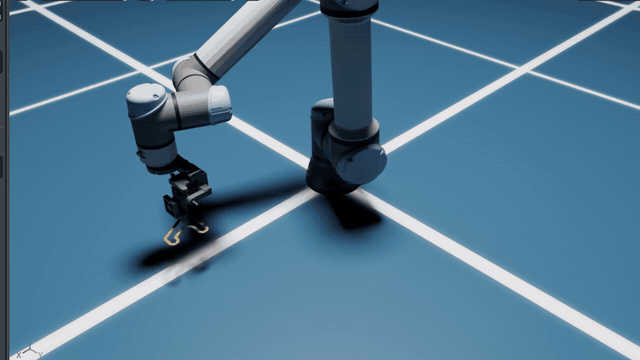
\includegraphics[width=0.92\linewidth]{figures/ur5e_replay.png}
\caption{Representative frame from the recorded UR5e mounted-extruder replay.
The orange curve is qualitative deposition visualization.}
\label{fig:isaac}
\end{figure}

\subsection{Automated software verification}

A fresh run of \software{python -m unittest discover -v} completed 55 tests in
\SI{7.006}{\second} with no failures.  The suite covers material conversion and
profile validation, metadata and extrusion conservation, generic robot-package
loading, synthetic global yaw selection, trajectory retiming, tolerance sweeps,
manipulability, approximate collision warnings, validation aggregation,
deposition scheduling and continuity, visual bead evolution, Isaac script
generation, and a capped end-to-end G-code export.

The evidence boundary matters.  The end-to-end test parses the full wall-hook
file but solves only ten capped waypoints for Panda and UR5.  Isaac tests compile
and inspect generated replay code and exercise selected visual-sink behavior
against fakes; they do not launch Isaac Sim or PhysX.  Passing these tests
supports software invariants and export structure, not physical print quality.

\Cref{tab:evidence} summarizes what is currently established and what remains
for a complete dynamic-repair paper.

\begin{table*}[!t]
\centering
\caption{Evidence boundary of the present manuscript.}
\label{tab:evidence}
\footnotesize
\begin{tabularx}{\textwidth}{@{}>{\raggedright\arraybackslash}p{0.14\textwidth}
  >{\raggedright\arraybackslash}X>{\raggedright\arraybackslash}X@{}}
\toprule
Area & Established here & Not yet established \\
\midrule
Path processing & Linear modal G-code, planar layers, metadata and extrusion conservation & Arc/spline expansion, non-planar normals, surface-relative replanning \\
Robot motion & Offline URDF IK, yaw selection, retiming, residual and limit reports & Certified real-time control, physical calibration, repeated hardware accuracy \\
Collision & Sampled capsule/AABB warnings & Continuous full-scene collision proof and safety certification \\
Deposition & Exact scheduled volume integration along measured simulated TCP; visual/PBD sinks & Calibrated rheology, thermal or curing physics, measured bead/repair quality \\
Simulation & Generated Isaac replay and qualitative prior recording & Retained current-version tracking logs and quantitative sim-to-real validation \\
Adaptation & Interfaces and data products suitable for later feedback & RGB-D perception, learned prediction, deformable surfaces, MPC, closed-loop repair \\
\bottomrule
\end{tabularx}
\end{table*}

\section{Discussion}

\subsection{What the integration enables}

The main value of the platform is traceability across layers that are often
implemented as unrelated scripts.  A positive G-code extrusion increment can
be followed from modal parsing, through simplification and subdivision, into a
material-profile volume, a retimed segment flow, and finally an emission along
the measured simulated TCP.  Machine-readable artifacts expose intermediate
states and allow failures to be localized to parsing, placement, IK, timing,
validation, export, tracking, or deposition.

Robot and material substitution are also separated.  The compact evaluation
used one path and volume command with three URDF packages; each robot retained
its own limits, home pose, TCP, and tolerance.  Conversely, one robot bundle can
be regenerated with a compatible material profile without changing its
directory structure or replay algorithm.  This separation is important for
future comparative studies, provided that G-code extrusion semantics are
explicitly compatible with the selected profile.

The measured-TCP deposition architecture avoids a common simulation shortcut.
Depositing along the commanded Cartesian path would hide articulation tracking
error and could draw material across a simulator discontinuity.  Sampling the
realized end-link hierarchy after the physics step makes the deposited geometry
respond to simulated robot motion.  Exact flow-boundary splitting and explicit
unrepresented-volume accounting then keep timing failures observable.

\subsection{Interpretation of the current results}

The common-patch study is a software planning comparison, not a robot
performance benchmark.  The packages have different degrees of freedom,
tolerances, home configurations, geometries, and TCPs; no repetitions or
physical measurements are available.  The archived UR5e case establishes that
a dense single-layer path was solved and retimed under the recorded model and
settings.  Neither case establishes calibration accuracy, bead geometry,
surface conformity, adhesion, structural performance, biocompatibility, or
safety.

The particle and geometric deposition modes serve different purposes.  PBD can
provide interactive material-like motion but is not a calibrated hydrogel or
polymer process model.  Geometric curves are inexpensive and their evolution is
fully inspectable, but a round radius cannot represent anisotropic flattening.
Quantitative deposition studies will require measured width, height, spreading,
sag, and volume data at controlled flow and speed, followed by held-out
validation rather than visual tuning.

\section{Limitations and Planned Extensions}

The gaps summarized in \Cref{tab:evidence} motivate near-term engineering work:
preserving an input manifest and hashes in
every output bundle, regenerating all reference artifacts with the current
exporter, recording desired-versus-measured tracking logs, expanding arc and
spline commands, assigning local surface normals, and replacing screening
collision geometry with a continuous model that includes the full workcell and
growing part.  Physical experiments must calibrate the bed and base frames,
nozzle TCP, payload, flow multiplier, and bead response.

The research roadmap then adds a stationary RGB-D sensor and dynamic repair
surface.  A short-horizon predictor would estimate future surface geometry or
quality from depth history, robot state, process state, and the planned local
toolpath.  A receding-horizon controller could compare local actions such as
speed changes, overlap changes, small tool offsets, normal adjustment, or an
additional pass.  Coverage, thickness deviation, surface error, remaining
defect volume, and overfill are candidate outcomes.  These ideas are included
only as a concrete direction for the next manuscript revision; no neural model,
training dataset, controller, wound model, or ship-panel model is evaluated in
the current repository.

\section{Conclusion}

The present \RPP{} connects conventional slicer intent to robot-aware planning
and simulator-ready deposition through explicit, inspectable stages.  It
preserves material and path semantics, solves configurable URDF robots with
nozzle-yaw redundancy, retimes trajectories against joint constraints, reports
kinematic and approximate collision diagnostics, and exports an Isaac replay
whose deposition follows measured simulated TCP motion.  A fresh common-input
case solved all 446 waypoints for Panda, UR5, and UR5e without reported joint
limit-rate violations or approximate collision warnings, and all 55 automated
tests passed.  These results establish a reproducible software foundation.  The
remaining scientific work is to add provenance-complete simulator experiments,
calibrated deposition and hardware validation, dynamic-surface perception, and
closed-loop repair-quality control.

% Split the final bibliography page into visually balanced columns.
\IEEEtriggeratref{11}
\bibliographystyle{IEEEtran}
\bibliography{references}

\end{document}
